\chapter{Field Models}

	\section{\texttt{PyGeopack}: Python wrapper for the Tsyganenko field models}

		This is a Python module for obtaining field vectors and traces of the Tsygenenko field models. It is a wrapper of a wrapper (see \ref{sectGeopack}). The latest code can be viewed and downloaded from here: \href{https://github.com/mattkjames7/PyGeopack}{https://github.com/mattkjames7/PyGeopack}.

		\subsection{Installation}

			The easiest way to install \texttt{PyGeopack} is using \texttt{pip}, e.g.:
			\begin{minted}{bash}
pip3 install PyGeopack --user
			\end{minted}
			for other installation methods, see the GitHub repo.

			At this point, it \textit{may} just work if you were to try to import it, but there's a reasonably good chance that the C++/Fortran code will need to be recompiled, in which case we need to ensure that there are compilers available to do this (see section \rec{sectSetup}). 

			One of the features of PyGeopack is that it can easily package together all of the geomagnetic/solar wind parameters that the models use so that when you request a trace or a field vector for a specific date and time, it will automatically try to find the appropriate parameters. This isn't strictly necessary for the models to work, as they will default to some fairly average parameters and they can be overridden manually. In order to be able to use this functionality, this module and the submodules which it relies on to collect the relevant data need to know where they can store the parameters. This means exporting a few environment variables (e.g. in \texttt{$\sim$/.bashrc}):
			\begin{minted}{bash}
export KPDATA_PATH=/path/to/kp
export OMNIDATA_PATH=/path/to/omni
export GEOPACK_PATH=/path/to/geopack/data				
			\end{minted}
			which are set as follows for me on SPECTRE:
			\begin{minted}{bash}
export KPDATA_PATH="/data/sol-ionosphere/mkj13/Kp"
export OMNIDATA_PATH="/data/sol-ionosphere/mkj13/OMNI"
export GEOPACK_PATH="/data/sol-ionosphere/mkj13/Geopack"			
			\end{minted}	
			
			Once that is done, it should work...
		
		\subsection{Usage}

			The first time this is imported, there is a good chance that it will attempt to recompile itself. There will be a lot of messages on the screen, but it should finish successfully. If it fails, double check that you have the required compilers installed, raise an issue on the GitHub page if the problem persists.

			If you would lke the latest model parameters, run the following:
			\begin{minted}{python}
import PyGeopack as gp
gp.Params.UpdateParameters(SkipWParameters=True)
			\end{minted}
			This may take a little time, depending on how much data it needs to download. It will take all of the data and compile it into one binary file $\sim$350 MiB in size, once this is done, it should be relatively quick loading the data into memory.

			The model field vectors can be returned using the \texttt{ModelField} function:
			\begin{minted}{python}
Bx,By,Bz = gp.ModelField(x,y,z,Date,ut,Model='T96',CoordIn='GSM',**kwargs)
			\end{minted}
			where \texttt{x}, \texttt{y} and \texttt{z} can be scalars or arrays of position, in units of Earth radii and in the coordinate system defined by the \texttt{CoordIn} keyword (\texttt{'GSE'|'GSM'|'SM'}). \texttt{Date} can be an array or scalar of date(s) in the format yyyymmdd, while \texttt{ut} is in hours from the start of the day. The models currently available are \texttt{'T89'}, \texttt{'T96'}, \texttt{'T01'} and  \texttt{'TS05'}.

			Traces are simple to produce and can be done a single trace at a time, or in batches, e.g.:
			\begin{minted}{python}
import numpy as np

#define a few starting positions for the traces
x = np.array([2.0,4.0,6.0,8.0])
y = np.array([0.0,0.0,0.0,0.0])
z = np.array([0.0,0.0,0.0,0.0])

#run the traces, return TraceField object
T = gp.TraceField(x,y,z,20221222,16.0)

#plot field traces
ax = T.PlotRhoZ()
			\end{minted}
			which should produce a plot similar to figure \ref{figGeopackTrace}.

			\begin{figure}
				\centering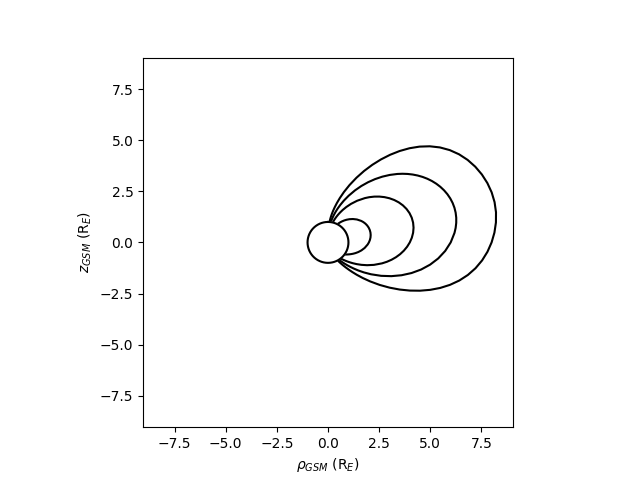
\includegraphics[width=\textwidth]{figures/ch03_geopacktrace.png}
				\caption{Example of field tracing using \texttt{PyGeopack}.
					\label{figGeopackTrace}}
			\end{figure}

			For more information on the keyword arguments please see the \href{https://github.com/mattkjames7/PyGeopack/blob/master/README.md}{readme}.

	\section{\texttt{geopack}: C++ wrapper for Tsyganenko field models}

		\label{sectGeopack}

		This is the code that \texttt{PyGeopack} calls, it provides a simple C-compatible interface for calculating field vectors, tracing and coordinate conversion. The C++ code in this library is used for configuring model parameters, determining footprints and providing a simple interface for the models, while the Fortran code currently provides field vectors, coordinate transforms and tracing.

		\subsection{Installation}

			This code can be installed as a linkable library (at least on POSIX systems):
			\begin{minted}{bash}
#clone the repo
git clone https://github.com/mattkjames7/geopack --recurse-submodules

#cd into it
cd geopack

#fetch the submodules if you forgot the 
#--recurse-submodules flag on the clone command
git submodule update --init --recursive

#compile it
make
sudo make install
			\end{minted}

			On Linux and MacOS the \texttt{sudo make install} command will place the header file at \texttt{/usr/local/include/geopack.h} and the shared object file at \texttt{/usr/local/lib/libgeopack.so}, unless the \texttt{PREFIX} keyword is set (by default \texttt{PREFIX=/usr/local}). If the \texttt{PREFIX} uses a custom path, then be sure to let the linker know where it exists, either by setting \texttt{LD\_LIBRARY\_PATH} or by using \texttt{-L} and \texttt{-I}.

			On Windows, run \texttt{compile.bat} to create \texttt{lib\\libgeopack.dll}.

		\subsection{Usage}
			
			To use this code with C and C++, the header file must be included, i.e.:
			\begin{minted}{cpp}
#include <geopack.h>
			\end{minted}
			and when compiling, the \texttt{-lgeopack} flag should be used to link to the library. 

			C and other languages such as Python should use the wrapper functions defined within the \texttt{extern "C" \{\}} section of \texttt{geopack.h}. This includes \texttt{ModelField()} for calculating model field vectors, \texttt{TraceField()} for field traces and a number of functions for coordinate conversion, e.g. \texttt{SMtoGSMUT()}. An example of how to trace a field line is in \texttt{geopack\tests\test.c}.

			C++ is able to use all of the functions declared in \texttt{geopack.h}, including the wrapper functions used by C. This means that direct usage of the \texttt{Trace} class is possible, an example of this is shown in \texttt{geopack\tests\test.cc}.
			

	\section{\texttt{libinternalfield}: C++ spherical harmonic model code}

		This library provides field vectors for spherical harmonic magnetic field models. It has a bunch of built in models from magnetized planets and a moon (Ganymede). This library is used by libjupitermag.

		\subsection{Installation}

			Compile and install in Linux and MacOS:

			\begin{minted}{bash}
#clone the repo
git clone https://github.com/mattkjames7/libinternalfield
		
#cd into it
cd libjupitermag
			
#compile it
make
sudo make install
			\end{minted}

			Or in Windows, run \texttt{compile.bat} to create \texttt{libinternalfield.dll}.

		\subsection{Usage}

			To use this library, the header should be included \texttt{#include <internalfield.h>} and the code should be compiled with the \texttt{-linternalfield} flag in order to link to the library.

			In C, we can use the \texttt{getModelFieldPointer()} to get a function pointer to the model we want to use, e.g.:
			\begin{minted}{c}
#include <stdio.h>
#include <internalfield.h>

int main() {

	printf("Testing C\n");
	
	/* try getting a model function */
	modelFieldPtr model = getModelFieldPtr("jrm33");
	double x = 10.0;
	double y = 10.0;
	double z = 0.0;
	double Bx, By, Bz;
	model(x,y,z,&Bx,&By,&Bz);

	printf("B = [%6.1f,%6.1f,%6.1f] nT at [%4.1f,%4.1f,%4.1f]\n",Bx,By,Bz,x,y,z);

	printf("C test done\n");

}
			\end{minted}

			C++ can use the \texttt{internalModel} object, e.g.:
			\begin{minted}{cpp}
#include <internal.h>

int main() {
    /* set current model */
    internalModel.SetModel("jrm09");

    /* set intput and output coordinates to Cartesian */
    internalModel.SetCartIn(true);
    internalModel.SetCartOut(true);

    /* input position (cartesian)*/
    double x = 35.0;
    double y = 10.0;
    double z = -4.0;

    /* output field */
    double Bx, By, Bz;
    internalModel.Field(x,y,z,&Bx,&By,&Bz);    
}
			\end{minted}


	\section{\texttt{vsmodel}: Python based Volland-Stern electric field model for Earth}
		
		This is a purely Python-based implementation of the Volland-Stern electric field model \citep{Volland1973,Stern1975}.

		\subsection{Installation}

		Use \texttt{pip}:
		\begin{minted}{bash}
pip3 install vsmodel --user
		\end{minted}

		\subsection{Usage}

			Electric field vectors can be determined using either cylindrical (\texttt{vsmodel.ModelE}) or Cartesian (\texttt{vsmodel.ModelCart}) coordinates (Solar Magnetic), e.g.:
			\begin{minted}{python}
import vsmodel

##### The simple model using Maynard and Chen ####
#the Cartesian model
Ex,Ey,Ez = vsmodel.ModelCart(x,y,Kp)

#the cylindrical model
Er,Ep,Ez = vsmodel.ModelE(r,phi,Kp)


#### The Goldstein et al 2005 version ####
#the Cartesian model, either by providing solar wind 
#speed (Vsw) and IMF Bz (Bz), or the equivalent E field (Esw)
Ex,Ey,Ez = vsmodel.ModelCart(x,y,Kp,Vsw=Vsw,Bz=Bz)
Ex,Ey,Ez = vsmodel.ModelCart(x,y,Kp,Esw=Esw)

#the cylindrical model
Er,Ep,Ez = vsmodel.ModelE(r,phi,Kp,Vsw=Vsw,Bz=Bz)
Er,Ep,Ez = vsmodel.ModelE(r,phi,Kp,Esw=Esw)
			\end{minted}
			where the \citet{Maynard1975} method uses the Kp index and the \citet{Goldstein2005} method uses Kp, solar wind speed and the $z$-component of the interplanetary magnetic field.

			The electric field magnitude and $\mathbf{E}\times\mathbf{B}$ velocity can be plotted in the Earth's equatorial plane:
			\begin{minted}{python}
import vsmodel
import matplotlib.pyplot as plt

plt.figure(figsize=(9,8))
ax0 = vsmodel.PlotModelEq('E',Kp=1.0,Vsw=-400.0,Bz=-2.5,
		maps=[2,2,0,0],fig=plt,fmt='%4.2f',scale=[0.01,10.0])
ax1 = vsmodel.PlotModelEq('E',Kp=5.0,Vsw=-400.0,Bz=-2.5,
		maps=[2,2,1,0],fig=plt,fmt='%4.2f',scale=[0.01,10.0])
ax2 = vsmodel.PlotModelEq('V',Kp=1.0,Vsw=-400.0,Bz=-2.5,
		maps=[2,2,0,1],fig=plt,scale=[100.0,10000.0])
ax3 = vsmodel.PlotModelEq('V',Kp=5.0,Vsw=-400.0,Bz=-2.5,
		maps=[2,2,1,1],fig=plt,scale=[100.0,10000.0])
ax0.set_title('$K_p=1$; $E_{sw}=-1$ mV m$^{-1}$')
ax2.set_title('$K_p=1$; $E_{sw}=-1$ mV m$^{-1}$')
ax3.set_title('$K_p=5$; $E_{sw}=-1$ mV m$^{-1}$')
ax1.set_title('$K_p=5$; $E_{sw}=-1$ mV m$^{-1}$')
plt.tight_layout()
			\end{minted}
			which would produce figure \ref{figVS}

			\begin{figure}
				\centering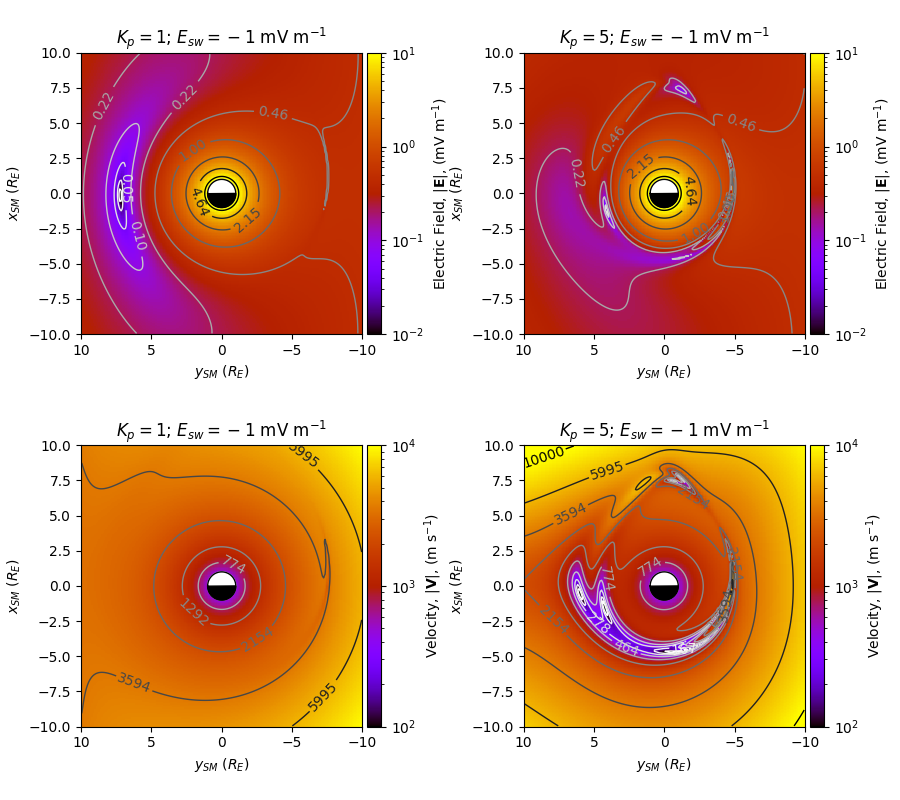
\includegraphics[width=\textwidth]{figures/ch03_vsmodel.png}
				\caption{Volland-Stern electric field (top plots) and $\mathbf{E}\times\mathbf{B}$ velocity (bottom plots). \label{figVS}}
			\end{figure}

	\section{\texttt{JupiterMag}: Python wrapper for Jovian field models}

		GitHub: \href{https://github.com/mattkjames7/JupiterMag.git}{https://github.com/mattkjames7/JupiterMag.git}

		Python wrapper for a collection of Jovian magnetic field models written in C++ (see \href{https://github.com/mattkjames7/libjupitermag.git}{libjupitermag}).
	
		This is part of a community code project :
		\href{https://lasp.colorado.edu/home/mop/missions/juno/community-code/}{Magnetospheres of the Outer Planets Group Community Code}

	
	\subsection{Requirements}
	
		For the Python code to run (without rebuilding the C++ backend), the following Python packages would be required:
		
		\begin{itemize}
			\item NumPy
			\item Matplotlib
			\item DateTimeTools
			\item RecarrayTools
			\item PyFileIO
		\end{itemize}
	
		All of which would be installed automatically if using \texttt{pip}.
	
		On some systems, the shared object files would need rebuilding before they can be loaded and accessed using Python. Upon the first import of the \texttt{JupiterMag} module, if the shared object/DLL fails to load then it will attempt to use a local C++ compiler to rebuild the binaries.
	
	\subsubsection{Linux}
	
		JupiterMag was built and tested primarily using Linux Mint 20.3 (based on Ubuntu 20.04/Debian). To rebuild the code, ensure that \texttt{g++}, \texttt{make}, and \texttt{ld} are installed.
	
	\subsubsection{Windows}
	
		This has been tested on Windows 10 (64-bit), other versions may also work. Requires \texttt{g++} and \texttt{ld} to work (these can be provided by TDM-GCC). This may or may not work with other compilers installed.
	
	\subsubsection{MacOS}
	
		This module has been tested on MacOS 11 Big Sur. It requires \texttt{g++}, \texttt{make}, and \texttt{libtool} to recompile (provided by Xcode).
	
	\subsection{Installation}
	
		Install using \texttt{pip3}:
	
		\begin{minted}{bash}
pip3 install JupiterMag --user
		\end{minted}
	
		Download the latest release (on the right $\rightarrow$ if you're viewing this on GitHub), then from within the directory where it was saved:
	
		\begin{minted}{bash}
pip3 install JupiterMag-1.0.0-py3-none-any.whl --user
		\end{minted}
	
		Or using this repo (replace "1.0.0" with the current version number):
	
		\begin{minted}{bash}
#pull this repo
git clone https://github.com/mattkjames7/JupiterMag.git
cd JupiterMag
	
#update the submodule
git submodule update --init --recursive
	
#build the wheel file
python3 setup.py bdist_wheel
#the output of the previous command should give some indication of
#the current version number. If it's not obvious then do
# $ls dist/ to see what the latest version is
pip3 install dist/JupiterMag-1.0.0-py3-none-any.whl --user
		\end{minted}
	
		I recommend installing \texttt{gcc} $\geq$ 9.3 (that's what this is tested with, earlier versions may not support the required features of C++).
	
		This module should now work with both Windows and MacOS.
	
	\subsubsection{Update an Existing Installation}
	
		To update an existing installation:
	
		\begin{minted}{bash}
pip3 install JupiterMag --upgrade --user
		\end{minted}
	
		Alternatively, uninstall then reinstall, e.g.:
	
		\begin{minted}{bash}
pip3 uninstall JupiterMag
pip3 install JupiterMag --user
		\end{minted}
	
	\subsection{Usage}
	
	\subsubsection{Internal Field}
	
		A number of internal field models are included (see \href{https://github.com/mattkjames7/libinternalfield/blob/main/README.md}{here} for more information) and can be accessed via the \texttt{JupiterMag.Internal} submodule, e.g.:
	
		\begin{minted}{python}
import JupiterMag as jm
	
#configure model to use VIP4 in polar coords (r,t,p)
jm.Internal.Config(Model="vip4",CartesianIn=False,CartesianOut=False)
Br,Bt,Bp = jm.Internal.Field(r,t,p)
	
#or use jrm33 in cartesian coordinates (x,y,z)
jm.Internal.Config(Model="jrm33",CartesianIn=True,CartesianOut=True)
Bx,By,Bz = jm.Internal.Field(x,y,z)
		\end{minted}
	
		All coordinates are either in planetary radii ($x,y,z,r$) or radians ($t,p$). All Jovian models here use $R_j=71,492$ km.
	
	\subsubsection{External Field}
	
		Currently, the only external field source included is the Con2020 field (see \href{https://github.com/gabbyprovan/con2020.git}{here} for the standalone Python code and \href{https://github.com/mattkjames7/libcon2020.git}{here} for more information on the C++ code used here as part of libjupitermag), other models could be added in the future.
		
		This works in a similar way to the internal field, e.g.:
		
		\begin{minted}{python}
#configure model
jm.Con2020.Config(equation_type='analytic')
Bx,By,Bz = jm.Con2020.Field(x,y,z)
		\end{minted}
	
	\subsubsection{Tracing}
	
		Field line tracing can be done using the \texttt{TraceField} object, e.g.
	
		\begin{minted}{python}
import JupiterMag as jm
	
#configure external field model prior to tracing
#in this case using the analytic Con2020 model for speed
jm.Con2020.Config(equation_type='analytic')
	
#trace the field in both directions from a starting position
T = jm.TraceField(5.0,0.0,0.0,IntModel='jrm09',ExtModel='Con2020')
		\end{minted}
	
		The above example will trace the field line from the Cartesian SIII position (5.0,0.0,0.0) ($R_j$) in both directions until it reaches the planet using the JRM09 internal field model with the Con2020 external field model. The object returned, \texttt{T}, is an instance of the \texttt{TraceField} class which contains the positions and magnetic field vectors at each step along the trace, along with some footprint coordinates and member functions which can be used for plotting.
	
		A longer example below can be used to compare field traces using just an internal field model (JRM33) with both internal and external field models (JRM33  + Con2020):
	
		\begin{minted}{python}
import JupiterMag as jm
import numpy as np
	
#be sure to configure external field model prior to tracing
jm.Con2020.Config(equation_type='analytic')
#this may also become necessary with internal models in the future, e.g.
#setting the model degree
	
#create some starting positions
n = 8
theta = (180.0 - np.linspace(22.5,35,n))*np.pi/180.0
r = np.ones(n)
x0 = r*np.sin(theta)
y0 = np.zeros(n)
z0 = r*np.cos(theta)
	
#create trace objects, pass starting position(s) x0,y0,z0
T0 = jm.TraceField(x0,y0,z0,Verbose=True,IntModel='jrm33',ExtModel='none')
T1 = jm.TraceField(x0,y0,z0,Verbose=True,IntModel='jrm33',ExtModel='Con2020')
	
#plot a trace
ax = T0.PlotRhoZ(label='JRM33',color='black')
ax = T1.PlotRhoZ(fig=ax,label='JRM33 + Con2020',color='red')
	
ax.set_xlim(-2.0,15.0)
ax.set_ylim(-6.0,6.0)
		\end{minted}
		
		The resulting objects T0 and T1 store arrays of trace positions and magnetic field vectors along with a bunch of footprints. The above code produces figure \ref{FigJMCT}.
		
		\begin{figure}[h]
			\centering
			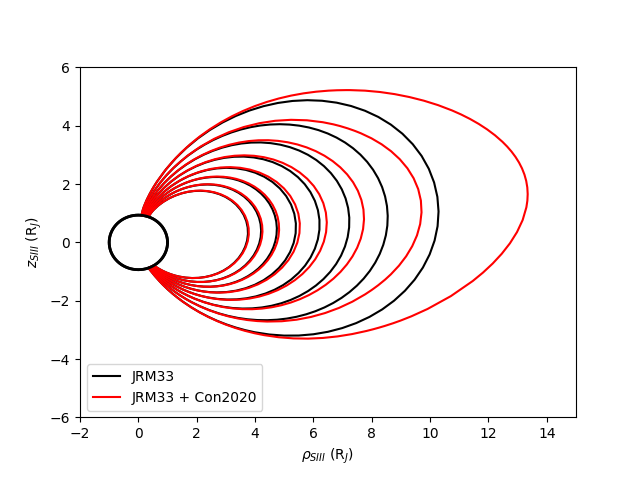
\includegraphics[width=0.7\linewidth]{figures/ch3_JMCompareTrace.png}
			\caption{Comparison between traces using only the internal field (black) and traces also using a magnetodisc model (red). \label{FigJMCT}}
		\end{figure}
	

	\section{\texttt{libjupitermag}: C++ library for field tracing in Jupiter's magnetosphere}

		GitHub: \href{https://github.com/mattkjames7/libjupitermag.git}{https://github.com/mattkjames7/libjupitermag.git}

		Code for obtaining magnetic field vectors and traces from within Jupiter's magnetosphere using various magnetic field models.

		This is part of a community code project :
		
		\href{https://lasp.colorado.edu/home/mop/missions/juno/community-code/}{Magnetospheres of the Outer Planets Group Community Code}
		
		This module forms part of the \href{https://github.com/mattkjames7/JupiterMag.git}{JupiterMag} package for Python.
		
	\subsection{Cloning and Building}
	
		This module requires a few submodules to be fetched, so the following command should clone everything:
	
		\begin{minted}{bash}
git clone --recurse-sumodules https://github.com/mattkjames7/libjupitermag.git
		\end{minted}
	
		This library requires \texttt{g++}, \texttt{make}, and \texttt{ld} (Linux) or \texttt{libtool} (Mac) in order to be compiled. On Windows, these tools can be provided by TDM-GCC.
	
		To build in Linux and Mac, simply run
	
		\begin{minted}{bash}
cd libjupitermag
make
#optionally install the library
sudo make install
		\end{minted}
	
		where the installation defaults to \texttt{/usr/local} but can be changed using the \texttt{PREFIX} argument, e.g.:
	
		\begin{minted}{bash}
sudo make install PREFIX=/usr
		\end{minted}
	
		It can also be uninstalled:
	
		\begin{minted}{bash}
make uninstall
		\end{minted}
	
		Under Windows powershell/command line:
	
		\begin{minted}{powershell}
cd libjupitermag
compile.bat
		\end{minted}
	
		or under Linux but building for Windows:
	
		\begin{minted}{bash}
cd libjupitermag
make windows
		\end{minted}
	
		After a successful build, a new library (\texttt{libjupitermag.so}) or DLL (\texttt{libjupitermag.dll}) should appear in the \texttt{lib/libjupitermag} directory.
	
	\subsection{Usage}
	
		The shared object library created by compiling this project should be accessible by various programming languages. This section mostly covers C++, other languages should be able to use the functions defined in the \texttt{extern "C"} section of the header file quite easily. For Python, it is straightforward to use \texttt{ctypes} to access this library, similarly, IDL could use the \texttt{CALL\_EXTERNAL} function.
	
	\subsubsection{Linking to the library}
	
		Here is a very basic example of how to link to the code using C++ and print the version of the library:
	
		\begin{minted}{cpp}
/* test.cc */
#include <stdio.h>
#include <jupitermag.h>
	
int main() {
	/* simply print the version of the library */
	printf("libjupitermag version: $%d.%d.%d\n",
			LIBJUPITERMAG_VERSION_MAJOR,
			LIBJUPITERMAG_VERSION_MINOR,
			LIBJUPITERMAG_VERSION_PATCH);
	return 0;
} 
		\end{minted}
	
		If the library was installed using \texttt{sudo make install}, then the library can be linked to during compiling time with:
	
		\begin{minted}{bash}
g++ test.c -o test -ljupitermag
		\end{minted}
	
		Otherwise, the header should be included using a relative or absolute path, e.g:
	
		\begin{minted}{cpp}
/* instead of this */
#include <jupitermag>
/* use something like this */
#include "include/jupitermag.h"
		\end{minted}
	
		then compile, e.g.:
	
		\begin{minted}{bash}
# absolute path
g++ test.cc -o test -L:/path/to/libjupitermag.so
	
# or relative path
g++ test.cc -o test -Wl,-rpath='$$ORIGIN/../lib/libjupitermag' -L ..lib/libjupitermag -ljupitermag
		\end{minted}
	
	\subsubsection{Calling Field Models}
	
		Internal field models can be called using the \texttt{InternalModel} object, e.g.:
	
		\begin{minted}{cpp}
#include <stdio.h>
#include <jupitermag.h>
	
int main () {
	/* create an instance of the object */
	InternalModel modelobj = InternalModel();
	
	/* set the model to use */
	modelobj.SetModel("jrm09");
	
	/* get the model vectors at some position */
	double x = 10.0, y = 0.0, z = 0.0;
	double Bx, By, Bz;
	modelobj.Field(x,y,z,&Bx,&By,&Bz);

	printf("B at [%f,%f,%f] = [%f,%f,%f]\n",x,y,z,Bx,By,Bz);
}
		\end{minted}
	
		There are also simple functions for each of the models included in the library, see the table below.
	
		\begin{table}[h]
			\centering
			\begin{tabular}{|l|l|l|l|}
				\hline
				Model & C String & Field Function & Reference \\
				\hline
				JRM33 & \texttt{jrm33} & \texttt{jrm33Field} & Connerney et al., 2022 \\
				JRM09 & \texttt{jrm09} & \texttt{jrm09Field} & Connerney et al., 2018 \\
				ISaAC & \texttt{isaac} & \texttt{isaacField} & Hess et al., 2017 \\
				VIPAL & \texttt{vipal} & \texttt{vipalField} & Hess et al., 2011 \\
				VIP4 & \texttt{vip4} & \texttt{vip4Field} & Connerney 2007 \\
				VIT4 & \texttt{vit4} & \texttt{vit4Field} & Connerney 2007 \\
				O4 & \texttt{o4} & \texttt{o4Field} & Connerney 1981 \\
				O6 & \texttt{o6} & \texttt{o6Field} & Connerney 2007 \\
				GSFC15evs & \texttt{gsfc15evs} & \texttt{gsfc15evsField} & Connerney 1981 \\
				GSFC15ev & \texttt{gsfc15ev} & \texttt{gsfc15evField} & Connerney 1981 \\
				GSFC13ev & \texttt{gsfc13ev} & \texttt{gsfc13evField} & Connerney 1981 \\
				Ulysses 17ev & \texttt{u17ev} & \texttt{u17evField} & Connerney 2007 \\
				SHA & \texttt{sha} & \texttt{shaField} & Connerney 2007 \\
				Voyager 1 17ev & \texttt{v117ev} & \texttt{v117evField} & Connerney 2007 \\
				JPL15ev & \texttt{jpl15ev} & \texttt{jpl15evField} & Connerney 1981 \\
				JPL15evs & \texttt{jpl15evs} & \texttt{jpl15evsField} & Connerney 1981 \\
				P11A & \texttt{p11a} & \texttt{p11aField} & \\
				\hline
				\multicolumn{4}{|l|}{\textbf{External Model}} \\
				\hline
				Con 2020 & \texttt{con2020} & \texttt{Con2020Field} & Connerney et al., 1981; Edwards et al., 2001; Connerney et al., 2020 \\
				\hline
			\end{tabular}
			\caption{Internal and External Field Models}
		\end{table}
		
	\subsubsection{Field Tracing}
	
		Field tracing can be done using the \texttt{Trace} object, e.g.:
	
		\begin{minted}{cpp}
#include <stdio.h>
#include <jupitermag.h>
#include <vector>
	
int main () {
	/* set initial position to start trace from (this can be an array
		for multiple traces) */
	int n = 1;
	double x0 = 5.0;
	double y0 = 0.0;
	double z0 = 0.0;
	int nalpha = 1;
	double alpha = 0.0;
	
	printf("Create field function vector\n");
	/* store the function pointers for the components of the
	model to be included in the trace */
	std::vector<FieldFuncPtr> Funcs;
	
	/* internal model */
	Funcs.push_back(jrm09Field);
	
	/* external model */
	Funcs.push_back(Con2020Field);
	
	/* initialise the trace object */
	printf("Create Trace object\n");
	Trace T(Funcs);
	
	/* add the starting positions for the traces */
	printf("Add starting position\n");
	T.InputPos(n,&x0,&y0,&z0);
	
	/* configure the trace parameters, leaving this empty will
	use default values for things like minimum and maximum step size */
	printf("Set the trace parameters \n");
	T.SetTraceCFG();
	
	/* set up the alpha calculation - the angles (in degrees) of each 
	polarization angle. This is generally used for ULF waves */
	printf("Initialize alpha\n");
	T.SetAlpha(nalpha,&alpha);    
	
	/* Trace */
	printf("Trace\n");
	T.TraceField();
	
	/* trace distance, footprints, Rnorm */
	printf("Footprints etc...\n");
	T.CalculateTraceDist();
	T.CalculateTraceFP();
	T.CalculateTraceRnorm();
	
	/* calculate halpha for each of the polarization angles 
	   specified above*/
	printf("H_alpha\n");
	T.CalculateHalpha();
}
		\end{minted}
		
		The above code traces along the magnetic field using the JRM09 internal and Con2020 external field models together. The trace coordinates and field vectors at each step can be obtained from the member variables \texttt{T.x\_}, \texttt{T.y\_}, \texttt{T.z\_}, \texttt{T.Bx\_}, \texttt{T.By\_}, and \texttt{T.Bz\_}, where each is a 2D array with the shape (\texttt{T.n\_},\texttt{T.MaxLen\_}), where \texttt{T.n\_} is the number of traces and \texttt{T.MaxLen\_} is the maximum number of steps allowed in the trace. The number of steps taken in each trace is defined in the \texttt{T.nstep\_} array.
		


	\section{\texttt{con2020}: Python implementation of Jupiter's magnetodisc model}

	\section{con2020}

	\href{https://zenodo.org/badge/doi/10.5281/zenodo.6959770.svg}{\includegraphics{https://zenodo.org/badge/doi/10.5281/zenodo.6959770.svg}} \\
	Python implementation of the Connerney et al., 1981 and Connerney et al., 2020 Jovian magnetodisc model. This model provides the magnetic field due to a "washer-shaped" current near to Jupiter's magnetic equator. This model code uses either analytical equations from Edwards et al., 2001 or the numerical integration of the Connerney et al., 1981 equations to provide the magnetodisc field, depending upon proximity to the disc along $z$ and the inner edge of the disc, $r_0$.
	
	For the IDL implementation of this model, see:
	\href{https://github.com/marissav06/con2020_idl}{https://github.com/marissav06/con2020_idl}
	
	Or for Matlab:
	\href{https://github.com/marissav06/con2020_matlab}{https://github.com/marissav06/con2020_matlab}
	
	A PDF documentation file is available here: \href{https://github.com/gabbyprovan/con2020/files/8869108/con2020_final_code_documentation_june9_2022.pdf}{con2020_final_code_documentation_june9_2022.pdf}. It describes the Connerney current sheet model and general code development (equations used, numerical integration assumptions, accuracy testing, etc.). Details specific to the Python code are provided in this readme file.
	
	These codes were developed by Fran Bagenal, Marty Brennan, Matt James, Gabby Provan, Marissa Vogt, and Rob Wilson, with thanks to Jack Connerney and Masafumi Imai. They are intended for use by the Juno science team and other members of the planetary magnetospheres community. Our contact information is in the documentation PDF file.
	
	\subsection{Installation}
	
	Install the module using \texttt{pip3}:
	
	\begin{minted}{bash}
pip3 install --user con2020
	
#or if you have previously installed using this method
pip3 install --upgrade --user con2020
	\end{minted}
	
	Or using this repo:
	
	\begin{minted}{bash}
#clone the repo
git clone https://github.com/gabbyprovan/con2020
cd con2020
	
#EITHER create a wheel and install (X.X.X is the current version number)
python3 setup.py bdist_wheel
pip3 install --user dist/con2020-X.X.X-py3-none-any.whl
	
#or directly install using setup.py
python3 setup.py insall --user
	\end{minted}
	
	\subsection{Usage}
	
	To call the model, an object must be created first using \texttt{con2020.Model()}, where the default model parameters, model equations used or coordinate systems of input and output can be altered using keywords, e.g:
	
	\begin{minted}{python}
import con2020
	
#initialize a model object with default parameters
def_model = con2020.Model()
	
#initialize a model which uses spherical polar coordinates for input and output
sph_model = con2020.Model(CartesianIn=False,CartesianOut=False)
	
#initialize a model with custom parameters (longhand)
cust_model0 = con2020.Model(mu_i_div2__current_parameter_nT=150.0,
						   	r0__inner_rj=9.5,
							d__cs_half_thickness_rj=3.1)
	
#equivalently, a custom parameter model (shorthand)
cust_model1 = con2020.Model(mu_i=150.0,r0=9.5,d=3.1)
	\end{minted}
	
	Once a model object is initialized, the model field can be obtained by calling the member function \texttt{Field()} and supplying input coordinates as three scalars, or three arrays (all of which are in right-handed System III), e.g.:
	
	\begin{minted}{python}
#Example 1: the model at a single Cartesian position (all in Rj)
x = 5.0
y = 10.0
z = 6.0
Bcart = def_model.Field(x,y,z)
#Result:
Bxyz=[15.57977074, 36.88229249, 63.02051163] nT
#Calculated using the default con2020 model keywords and the hybrid approximation.
	
#Example 2: the model at an array of positions of spherical polar coordinates
r = np.array([10.0,20.0])					#radial distance in Rj
theta = np.array([30.0,35.0])*np.pi/180.0	#colatitude in radians 
phi = np.array([90.0,95.0])*np.pi/180.0	#east longitude in radians
Bpol = sph_model.Field(r,theta,phi)
#Result:
Spherical polar Brtp =[63.32354453 ,31.15790459], [-21.01051861 , -6.86773727], [-3.61151705, -2.72626057] nT
Cartesian       Bxyz =[3.61151705, 1.6486016], [13.4661294,  12.43672946], [65.34505753, 29.46223351] nT
#Calculated using the default con2020 model keywords and the hybrid approximation.
	\end{minted}
	
	The output will be a \texttt{numpy.ndarray} with a shape \texttt{(n,3)}, where \texttt{n} is the number of input coordinates, \texttt{B[:,0]} corresponds to either \texttt{Bx} or \texttt{Br}; \texttt{B[:,1]} corresponds to \texttt{By} or \texttt{Btheta}; and \texttt{B[:,2]} corresponds to either \texttt{Bz} or \texttt{Bphi}.  A full list of model keywords is shown below:
	
	\begin{table}[h]
	\centering
	\begin{tabular}{|l|l|l|l|}
	\hline
	\textbf{Keyword (long)} & \textbf{Keyword (short)} & \textbf{Default Value} & \textbf{Description} \\ \hline
	\texttt{mu\_i\_div2\_\_current\_parameter\_nT} & \texttt{mu\_i} & \texttt{139.6}* & Current sheet current density in nT. \\ \hline
	\texttt{i\_rho\_\_radial\_current\_MA} & \texttt{i\_rho} & \texttt{16.7}* & \begin{tabular}[c]{@{}l@{}}\textsuperscript{†}Radial current intensity in MA \\ from Connerney et al 2020.\end{tabular} \\ \hline
	\texttt{r0\_\_inner\_rj} & \texttt{r0} & \texttt{7.8} & Inner edge of the current sheet in Rj. \\ \hline
	\texttt{r1\_\_outer\_rj} & \texttt{r1} & \texttt{51.4} & Outer edge of the current sheet in Rj. \\ \hline
	\texttt{d\_\_cs\_half\_thickness\_rj} & \texttt{d} & \texttt{3.6} & Current sheet half thickness in Rj. \\ \hline
	\texttt{xt\_\_cs\_tilt\_degs} & \texttt{xt} & \texttt{9.3} & Tilt angle of the current sheet away from the SIII \textit{z}-axis in degrees. \\ \hline
	\texttt{xp\_\_cs\_rhs\_azimuthal\_angle\_of\_tilt\_degs} & \texttt{xp} & \texttt{155.8} & (Right-Handed) Longitude towards which the current sheet is tilted in degrees. \\ \hline
	\texttt{equation\_type} &  & \texttt{'hybrid'} & \begin{tabular}[c]{@{}l@{}}Which method to use, can be: \\ \texttt{'analytic'} - use only the analytical equations \\ \texttt{'integral'} - numerically integrate the equations \\ \texttt{'hybrid'} - a combination of analytical and integration (default)\end{tabular} \\ \hline
	\texttt{error\_check} &  & \texttt{True} & Check errors on inputs the the \texttt{Field()} member function - set to \texttt{False} at your own risk for a slight speedup. \\ \hline
	\texttt{CartesianIn} &  & \texttt{True} & If \texttt{True} (default) then the input coordinates are expected to be in Cartesian right-handed SIII coordinates. If \texttt{False} then right-handed spherical polar SIII coordinates will be expected. \\ \hline
	\texttt{CartesianOut} &  & \texttt{True} & If \texttt{True} the output magnetic field components will be in right-handed Cartesian SIII coordinates. If \texttt{False} then the output will be such that it has radial, meridional and azimuthal components. \\ \hline
	\texttt{azfunc} &  & \texttt{'connerney'} & Which model to use for the azimuthal component of the magnetodisc current: \texttt{'connerney'} - use Connerney et al., 2020 model; \texttt{'lmic'} - use the Leicester magnetosphere-ionosphere coupling (L-MIC) model (Cowley et al., 2005, 2008). \\ \hline
	\texttt{DeltaRho} &  & \texttt{1.0} & Scale length over which smoothing is done in the $\rho$ direction Rj. \\ \hline
	\texttt{DeltaZ} &  & \texttt{0.1} & Scale length over which smoothing is done in the $z$ direction. \\ \hline
	\texttt{g} &  & \texttt{417659.3836476442} & \textsuperscript{§}Magnetic dipole parameter, nT \\ \hline
	\texttt{wO\_open} &  & \texttt{0.1} & \textsuperscript{§}Ratio of plasma to Jupiter's angular velocity on open field lines. \\ \hline
	\texttt{wO\_om} &  & \texttt{0.35} & \textsuperscript{§}Ratio of plasma to Jupiter's angular velocity in the outer magnetosphere. \\ \hline
	\texttt{thetamm} &  & \texttt{16.1} & \textsuperscript{§}Colatitude of the centre of the middle magnetosphere, where the plasma transitions from corotating to sub-corotating, °. \\ \hline
	\texttt{dthetamm} & & \texttt{0.5} & \textsuperscript{§}Colatitude range over which the transition from inner to outer magnetosphere occurs, °. \\ \hline
	\texttt{thetaoc} &  & \texttt{10.716} & \textsuperscript{§}Colatitude of the centre of the open-closed field line boundary, °. \\ \hline
	\texttt{dthetaoc} & & \texttt{0.125} & \textsuperscript{§}Colatitude range of the open-closed field line boundary, °. \\ \hline
	\end{tabular}
	\end{table}
	
	*Default current densities used here are averages provided in Connerney et al., 2020 (see Figure 6), but can vary from one pass to the next. Table 2 of Connerney et al., 2020 provides a list of both current densities for 23 out of the first 24 perijoves of Juno.
	
	\textsuperscript{†} This is only applicable for the Connerney et al., 2020 model for $B_{\phi}$.
	
	\textsuperscript{§} These parameters are used to configure the L-MIC model for $B_{\phi}$.
	
	The \texttt{con2020.Test()} function should produce figure \ref{Figcon20202Test}:
	
	\begin{figure}
		\centering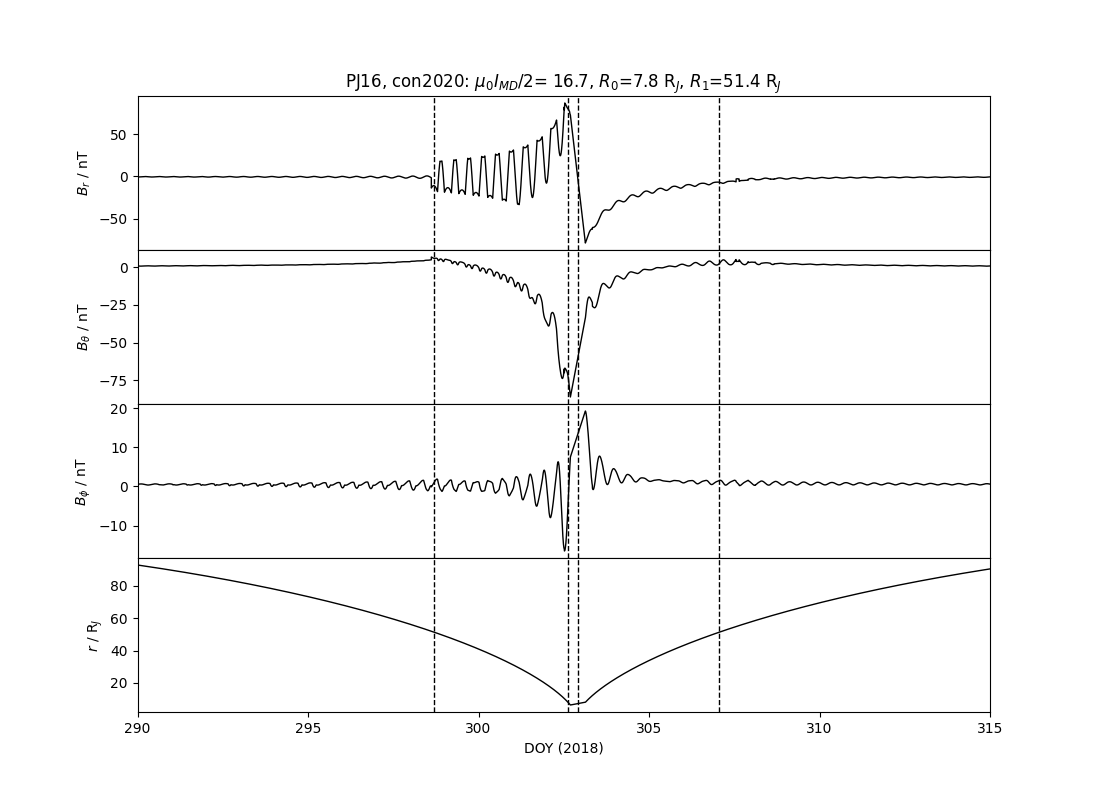
\includegraphics[width=0.8\textwidth]{figures/ch3_con2020Test.png}
		\caption{Test of \texttt{con2020} code on a Juno orbit.\label{Figcon20202Test}}
	\end{figure}


	\section{\texttt{libcon2020}: C++ implementation of Jupiter's magnetodisc model}

	\section{\texttt{jrm33}: The JRM33 model in Python}

	\section{\texttt{jrm09}: The JRM09 model in Python}

	\section{\texttt{vip4model}: The VIP4 model in Python}
	